
\chapter{Sistemas de ecuaciones lineales: método de Gauss}
\chaptermark{S.E.L.: MÉTODO DE GAUSS}	

\section[Sistemas de dos ecuaciones lineales con dos incógnitas]{Sistemas de dos ecuaciones lineales con dos incógnitas}\sectionmark{Sistemas 2ecc-2incog}
\sectionmark{Sistemas 2ecc-2incog}
\begin{defi}
Una `ecuación lineal' con dos incógnitas es una relación de la forma: $ax+by=c$, con $a,b,c \in \mathbb R$. $x$ e $y$ son las incógnitas	.
Cualquier par de valores $(\alpha, \beta)$ que verifiquen la ecuación se llaman `solución' de la misma.
\end{defi}
\vspace{-3mm}
\noindent \small{--- Cualquier ecuación lineal con dos incógnitas, $ax+by=c$, admite siempre infinitas soluciones. Hay que dar valor a una incógnita y calcular el valor correspondiente en la otra.}

\noindent \small{--- Interpretación geométrica: si representamos en el plano todas las infinitas soluciones de cualquier ecuación lineal con dos incógnitas, $ax+by=c$, obtenemos una `recta' en el plano.}

\small{Vamos a empezar considerando sistemas de \textbf{2} ecuaciones lineales con \textbf{2} incógnitas. 
$\begin{cases}a_1x+b_1y=c_1\\a_2x+b_2y=c_2\end{cases}; \; a_i,b_i$ son los coeficientes y $c_i$ los términos independientes ($i=\{1,2\}$)}
\begin{defi}
Según sean las soluciones del sistema de ecuaciones lineales con dos incógnitas, éstos se clasifican en:	
\begin{enumerate}
\item \small{SISTEMA COMPATIBLE DETERMINADO (SCD): Solución única.}

\small{ejemplo: $\begin{cases} x-y=-3 \\2x+y=6 \end{cases} $
$\to \quad  \begin{matrix} 
\text{ sumando: } 
\\ 3x=3\;\to \;    \boldsymbol{x=1; \; y=4}
\end{matrix}$}

\small{Interpretación geométrica: las dos rectas que forman el sistema son secantes, ($r\cap s$), se cortan en un punto, el $(1,4)$.}
\item \small{SISTEMA COMPATIBLE INDETERMINADO (SCI): Infinitas soluciones.}

\small{ejemplo: $\begin{cases} x-y=-3 \\2x-2y=-6 \end{cases} \to \; \; \begin{matrix}  (1^a ec)(2)-(2^a ec) \\  0x=0;\;   \boldsymbol{x=\lambda} \to  \boldsymbol{y=3+\lambda} \\ \forall \lambda \in \mathbb R; \; \infty \text{ soluciones}\end{matrix}$	}

\small{Interpretación geométrica: las dos rectas que forman el sistema son coincidentes ($r \equiv s$), tienen todos ($\infty$) puntos en común.}
\item \small{SISTEMA INCOMPATIBLE (SI): No hay ninguna solución.}

\small{ejemplo: $\begin{cases} x-y=-3 \\2x-2y=5 \end{cases} \to \; \; \begin{matrix}  (1^a ec)(2)-(2^a ec) \\  0x=-8;\;   \boldsymbol{\nexists \; x}\; \to  \boldsymbol{\nexists \;  y} \end{matrix}$}	

\small{Interpretación geométrica: las dos rectas que forman el sistema son paralelas ($r \parallel s$), no tienen ningún punto en común.}
\end{enumerate}
\end{defi}

	\begin{figure}[H]
		\centering
		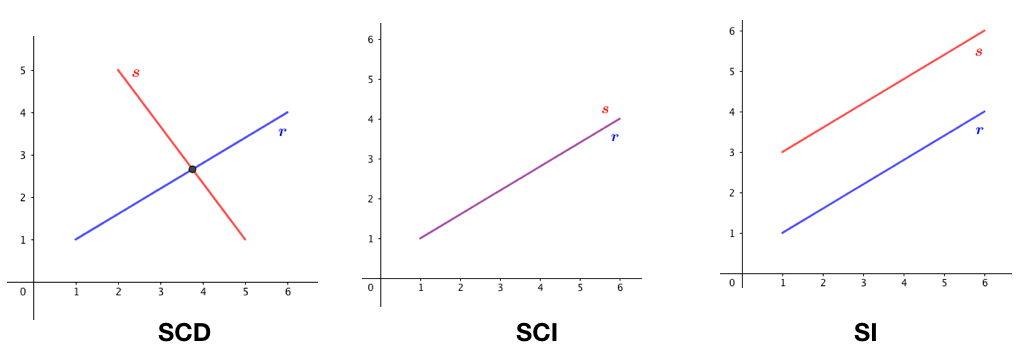
\includegraphics[width=1\textwidth]{imagenes/imagenes01/T01IM02.png}
	\end{figure}


\noindent \textbf{Forma matricial de un sistema de dos ecuaciones con dos incógnitas}
\vspace{4mm}

Aunque dedicaremos en un próximo capítulo a las matrices, de momento nos bastará considerar una matriz como un rectángulo que contiene números. Así, un Sistema de Ecuaciones Lineales (en adelante un SEL) lo podremos escribir, escribiendo en cada fila solamente los coeficientes de las ecuaciones y, a la derecha, separada por una barra vertical, |, los términos independientes. En la segunda fila se escribirán los coeficientes de la segunda ecuación y, a la derecha, su término independiente. En este caso usaremos una matriz de dos filas (ecuaciones) con tres columnas (dos para os coeficientes de las incógnitas  y la tercera columna para los términos independientes).

\vspace{4mm} \centerline{$\boxed{\; \begin{cases}a_1x+b_1y=c_1\\a_2x+b_2=c_2\end{cases} \Leftrightarrow 
\left[
\begin{matrix}
\; a_1&b_1\\
\; a_2&b_2	
\end{matrix}
\right|
\left.
\begin{matrix}
c_1\\c_2	
\end{matrix}
\right]\;} \; $
$\begin{matrix}\text{ Forma matricial de un S }\\\text{de dos E L con dos incog.}\end{matrix}$}

\vspace{4mm} $a_1, b_1, a_2, b_2$ son los coeficientes; $c_1, c_2$ son los términos independientes.

\section[Sistemas de Ecuaciones Lineales]{Sistemas de Ecuaciones Lineales}\sectionmark{SEL}
\sectionmark{SEL}

\begin{defi}
Se llama `Sistema de m-Ecuaciones Lineales con n-incógnitas' (SEL) a todo conjunto de relaciones de la forma:

\vspace{4mm}

\centerline{$\boxed{\; \begin{cases}
\;\; a_{11} x_1 + a_{12} x_2 + \cdots + a_{1j} x_j+ \cdots + a_{1n} x_n & = b_1\; \\
\;\; a_{21} x_1 + a_{22} x_2 + \cdots + a_{2j} x_j+ \cdots + a_{2n} x_n & = b_2\; \\
\;\; \cdots \quad \cdots \quad \cdots 	\quad \cdots \quad \cdots \quad \cdots \quad \cdots \quad \cdots & \cdots \\
\;\; a_{i1} x_1 + a_{i2} x_2 + \cdots + a_{ij} x_j+ \cdots + a_{in} x_n & = b_i\; \\
\;\; \cdots \quad \cdots \quad \cdots 	\quad \cdots \quad \cdots \quad \cdots \quad \cdots \quad \cdots & \cdots \\
\;\; a_{m1} x_1 + a_{m2} x_2 + \cdots + a_{mj} x_j+ \cdots + a_{mn} x_n & = b_m\; \\
\end{cases}}$}	
\end{defi}

\vspace{4mm} 

La primera fila son los coeficientes de las n-incógnitas y el término independiente de la primera ecuación. La segunda fila, la segunda ecuación, ... En la primera columna aparecen los coeficientes de la primera incógnita, en la segunda columna los coeficientes de la segunda incógnita, ... En la columna m+1 aparecen los términos independientes de las m-ecuaciones. Así, $a_{ij}$ es el coeficiente de la ecuación-i que acompaña a la incógnita-j.


\begin{myblock}{Forma matricial para representar un SEL}
\centerline{
$\left[ \begin{matrix}
\; a_{11} & a_{12} & \cdots & a_{1j} & \cdots & a_{1n} \;  \\
\; a_{21} & a_{22} & \cdots & a_{2j} & \cdots & a_{2n} \;  \\
\; \vdots & \vdots & \ddots & \vdots & \ddots & \cdots \;  \\
\; a_{i1} & a_{i2} & \cdots & a_{ij} & \cdots & a_{in} \;  \\
\; \vdots & \vdots & \ddots & \vdots & \ddots & \cdots \;  \\
\; a_{m1} & a_{m2} & \cdots & a_{mj} & \cdots & a_{mn} \;  
\end{matrix} \right.$
$\left| \begin{matrix}
\; b_1 \; \\
\; b_2 \;  \\
\; \vdots \; \\
\; b_i \; \\
\; \vdots \; \\
\; b_m \; 	
\end{matrix} \right]$
}
\end{myblock}


De nuevo, para cada $a_{ij}$, el subíndice-i hace referencia a la ecuación-i y el subíndice-j a la incógnita-j: $\; 1\le i\le m;\;$, m ecuaciones ; $ \; 1\le j \le n \;$, n-incógnitas.

\begin{defi}
Decimos que la n-tupla \textcolor{gris}{(conjunto de n números ordenados)} de números reales $(\alpha_1, \alpha_2, \alpha_3, \cdots, \alpha_n)$ son `solución' del SEL si sustituidas en él se satisfacen todas sus ecuaciones. 	
\end{defi}

\begin{defi}.
\begin{myblock}{Atendiendo a las soluciones, un SEL puede ser:}
$\begin{cases}
\text{COMPATIBLE (con solución)	} \; \; 	\to \; \begin{cases}
\text{DETERMINADO (Sol.única)} \\
\text{INDETREMINADO } (\infty \text{ sol.})
\end{cases}
\\
\text{INCOMPATIBLE (sin solución)} 	 \; \begin{matrix}
\text{ } \\
\text{}
\end{matrix}

\end{cases}$
\end{myblock}	
\end{defi}
\begin{defi}
	'`Resolver' un SEL es encontrar todas sus soluciones o advertir de que el sistema carece de soluciones.
\end{defi}

\section{Sistemas equivalentes}
\begin{defi}
Dos sistemas de ecuaciones lineales con el mismo número de incógnitas (aunque no tengan el mismo número de ecuaciones) se dice que son `equivalentes' si tienen las mismas soluciones, es decir, cualquier solución del primer sistema también lo es del segundo y viceversa.	
\end{defi}
\begin{teor}
Las siguientes transformaciones elementales realizadas a un SEL dan lugar a otro equivalente:

\begin{itemize}
\item Cambiar de orden las ecuaciones del sistema.
\item Multiplicar toda la ecuación (los dos miembros) por un número distinto de cero.
\item Sustituir una ecuación del sistema por ella misma más otra cualquiera multiplicada por un número cualquiera.
\item Sustituir una ecuación del sistema por ella misma multiplicada por un `numero distinto de cero' más otras ecuaciones multiplicadas por otros números. \textcolor{gris}{!`Ojo!, la ecuación a sustituir no puede estar multiplicada por cero, sería como cargarse una ecuación del sistema.}	
\end{itemize}
	
\end{teor}


\section[Resolución de SEL: Método de Gauss]{Resolución de SEL: Método de Gauss}\sectionmark{Método de Gauss}
\sectionmark{Método de Gauss}


El método de Gauss consiste en aplicar transformaciones a las ecuaciones (filas de números en la representación matricial) hasta obtener un sistema “triangular” (todos los coeficientes por debajo de la diagonal son cero) y, entonces, despejar en cascada (de abajo hacia arriba). Si nos aparece una trivialidad, $0=0$, se tacha y se prescinde de esa fila o ecuación (no aporta ninguna información al sistema); si llegamos a una incongruencia (incompatibilidad) $3=0$, p.e., tenemos un SI (sin solución). 

Este método está formado por varios pasos (m-1 pasos de las m-1 ecuaciones en que hay que buscar ceros por debajo de la diagonal): 

--- el primer paso consiste en combinar cada una de las ecuaciones $2, 3, \cdots, m$ con la ecuación $1$ para que todos sus primeros coeficientes sean cero ($a_{21}=a_{31}=\cdots=a_{m1}=0)$.

--- el segundo paso consiste en hacer que por debajo de la segunda fila, todos los segundos coeficientes del resto de ecuaciones sean cero, combinando cada ecuación $3, 4, \cdots , ,$ con la $2$ para conseguir que $a_{32}=a_{42}=\cdots=a_{m2}=0$.

--- y así hasta conseguir triangularizar la matriz, que por debajo de la diagonal todos los elementos sean ceros. 
				
	\begin{figure}[H]
		\centering
		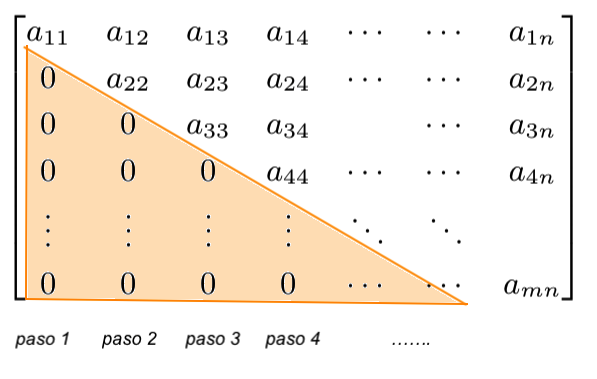
\includegraphics[width=0.7\textwidth]{imagenes/imagenes01/T01IM05.png}
	\end{figure}				
				
Cuando se llega a una ecuación con más de una incógnita se elige una de ellas y a las otras se les da valores arbitrarios (parámetros $\lambda, \mu, ...$) y se sigue despejando en función de éstos. Para ello:
				
\begin{teor}{Transformaciones de Gauss:} En la representación matricial de un SEL está permitido (da lugar a otra ecuación equivalente):
		
	\hspace{3mm} \colorbox{LightYellow}{* multiplicar una ecuación por un número distinto de cero.}
		
	\hspace{3mm}  \colorbox{LightYellow}{* Sustituir una ecuación por ella misma más otra  multiplicada} 
	
	\hspace{3mm} \colorbox{LightYellow}{ por un número.}
		
\noindent !`ASTUCIA!: se puede cambiar el orden de las ecuaciones y las incógnitas (advirtiéndolo en este último caso). Lo más conveniente es que el número con el que combinar, `pivote', sea $1$ ò $-1$, si es posible. En caso de que el coeficiente con el que pivotar sea cero, o bien cambiamos de orden las ecuaciones o sustituimos ésta por una combinación de ella con alguna otra de modo que el pivote sea distinto de cero.
\end{teor}



A continuación veremos unos ejemplos de resolución de sistemas de ecuaciones lineales por el método de Gauss.

\begin{ejem}.

$\begin{cases}
x-2y-2z&=-3\\2x-3y+4z&=4\\5x-y+3z&=16	
\end{cases} \to \left[ \begin{matrix}
 1&-2&-2\\2&-3&4\\5&-1&3	
 \end{matrix}\right. 
 \left| \begin{matrix}
 -3\\4\\16	
 \end{matrix}\right] \; \underrightarrow {(1*)} \;  
 \left[ \begin{matrix}
 1&-2&-2\\0&1&8\\0&9&13	
 \end{matrix}\right. 
 \left| \begin{matrix}
 -3\\10\\31	
 \end{matrix}\right] \; \underrightarrow {(2*)} \; $
 
 $
  \left[ \begin{matrix}
 1&-2&-2\\0&1&8\\0&0&-59	
 \end{matrix}\right. 
 \left| \begin{matrix}
 -3\\10\\-59	
 \end{matrix}\right] \;  \Rightarrow  \; \begin{cases}
 x-2y-2z=-3\\ y+8z=10\\-59z=-59	
 \end{cases}$

En el paso (1*) --primer paso del método de Gauss-- hemos combinado las ecuaciones segunda y tercera con la primera para conseguir los dos ceros de la primera columna ($2^a\to 2^a-2\cdot 1^a; \; \; 3^a\to 3^a-5\cdot 1^a$). En el paso (2*) --segundo paso del método de Gauss-- combinamos la tercera ecuación con la segunda para conseguir el cero de la tercera columna \textcolor{gris}{(ojo, combinamos 3$^a$ con 2$^a$ , no con 1$^a$, que desharíamos el cero anteriormente conseguido)}, la combinación elegida en este caso ha sido $3^a \to 3^a - 9\cdot 2^a$. \textcolor{gris}{Estos pasos no será necesarios explicarlos así como tampoco lo será reescribir el sistema de ecuaciones escalonado al que llegamos}. Con ello hemos conseguid un sistema `escalonado' y (sin necesidad de volver a escribir el sistema de ecuaciones lineales obtenido) nos ponemos a despejar en `cascada', de abajo hacia arriba: 

Leyendo la última ecuación: $[\; 0 \quad 0 \quad -59 \;\;  | \; \; -59 ] \to  -59z=-59 \Rightarrow \boldsymbol{z=1}$ 

Subimos un peldaño en la cascada y, con el valor encontrado para $x$, leemos la segunda ecuación: $[\; 0\quad 1 \quad 8 \; \; | \; \; 10] \to y+8z=10; \; y+8\cdot 1=10 \Rightarrow \boldsymbol{y=2}$

Por último, subimos a la primera ecuación y leemos: $[\; 1\quad -2\quad -2 \; \; | \; \; -3 ] \to x-2y-2z=-3 ; \; x -2\cdot 2-2\cdot 1=-3 ; \; x-4-2=-3 \rightarrow \boldsymbol{x=3}$

Solución única: $\boldsymbol{x=3;\;  y=2; \; z=1}$, \textbf{solución única}, \textbf{SDC} (sistema compatible y determinado).
\end{ejem}

\begin{ejem}.

$\begin{cases}
x-y+3z&=4\\2x-y-z&=6\\3x-2y+2z&=10	
\end{cases} \to \left[ \begin{matrix}
 1&-1&3\\2&-1&-1\\3&-2&2	
 \end{matrix}\right. 
 \left| \begin{matrix}
 4\\6\\10	
 \end{matrix}\right] \; \underrightarrow {(1*)} \;  
 \left[ \begin{matrix}
 1&-1&3\\0&1&-7\\0&1&-7	
 \end{matrix}\right. 
 \left| \begin{matrix}
 4\\-2\\-2	
 \end{matrix}\right] \; \underrightarrow {(2*)} \; $
 
 $
  \left[ \begin{matrix}
 1&-1&3\\0&1&-7\\ 0&0&0
 \end{matrix}\right. 
 \left| \begin{matrix}
 4\\-2\\0	
 \end{matrix}\right] \;  \Rightarrow  \; \begin{cases}
 x-y+3z=4\\ y-7z=-2\\0z=0	
 \end{cases}$
 
  \textcolor{gris}{$1*)\;\; 2ec \to 2ec  -  2\cdot 1ec; \; \; 3ec\to 3ec - 5\cdot 1ec; \quad 2*)\; \; 3ec \to 3ec  -  2ec $}


La última ecuación: $[\; 0\quad 0\quad 0 \; \; |\;\;  0\;]$ es lo que en matemáticas llamamos una `trivialidad' ($0\cdot z=0$), no aporta ninguna información y la eliminamos del sistema:

$  \left[ \begin{matrix}
 1&-1&3\\0&1&-7\\ \text{\textst{ 0 }} & \text{\textst{ 0 }} & \text{\textst{ 0 }}
 \end{matrix}\right. 
 \left| \begin{matrix}
 4\\-2\\ \text{\textst{ 0 }}	
 \end{matrix}\right] $


Leyendo ahora la última ecuación que ha quedado: $y-7z=-2$. Para resolver una ecuación con más de una incógnita, hay que elegir una de ellas, la $y$ por ejemplo y dar valores a las otras, la $z$ en este caso. En el problema que nos ocupa (método de Gauss para resolver SEL) lo que haremos es `parametrizar' las otras incógnita, $z$ en el ejemplo, del siguiente modo: $\;z=\lambda\; \; \forall \lambda \in \mathbb R$ e ir despejando el resto de incógnitas en función de estos parámetros:



$\;z=\lambda\; \; \forall \lambda \in \mathbb R \to \; $, última ecuación $\; y-7z=-2; \; y-7\lambda=-2 \Rightarrow y=-2+7\lambda\; $. Subimos un peldaño y vamos a la primera ecuación: $\; x-y+3z=4 \to x-(-2+7\lambda)+3\lambda=4 \Rightarrow x=2+4\lambda$



Las soluciones son: $\boldsymbol{\; x=2+4\lambda; \; \; y=-2+7\lambda; \; \; z=\lambda \;} $, como esto es  $\boldsymbol{\; \forall \lambda \in \mathbb R\;}$, tenemos \textbf{infinitas soluciones: SCI} (Sistema compatible Indeterminado)

Por ejemplo, si $\lambda=0 \to x=2; \; y=-2; \; z=0$ es una solución del sistema, la terna de números $(2,-2,0)$, en ese orden, son verifican todas las ecuaciones del sistema (x el primer número, y el segundo y z el tercero, de la terna). Para, p.e., $\lambda=-2 \to (-6,-16,-2)$, también lo es y así, como valores de $\lambda \in \mathbb R$ hay $\infty$, se pueden obtener las infinitas soluciones del mismo.

?`Es $(2,3,-1)$ solución del sistema?. Si lo fuese, $z=-1=\lambda \to x=-2\neq 2; \; y=-9\neq 3$. No, $(2,3,-1)$  no es solución del sistema.

?`Es $(32, 47, 7) $ solución del sistema? $\to z=7=\lambda \to x=32\; \; y=47$. Sí lo es.

?`¿Que deben valer $m$ y $n$ para que $(4,m,n)$ sea solución del sistema? Dicho de otro modo, Si $x=4$ es una de las soluciones del sistema, ?`qué vales las otras? Como $x=2+4\lambda=4 \to \lambda = \frac 1 /2 \Rightarrow y=-2+\frac 7 2=\frac 3 2; \; z=\frac 1 2$.
\end{ejem}

\begin{ejem}.

$\begin{cases}
2x-y+3z&=6\\4x-2y+6z&=9\\x-y+z&=3	
\end{cases} \to \left[ \begin{matrix}
 2&-1&3\\4&-2&6\\1&-1&1	
 \end{matrix}\right. 
 \left| \begin{matrix}
 \; 6\\\; 9\\\; 3	
 \end{matrix}\right] \;\underrightarrow {(1*)} \;  
 \left[ \begin{matrix}
 1&-1&1\\2&-1&3\\4&-2&6	
 \end{matrix}\right. 
 \left| \begin{matrix}
 \; 3\\\; 6\\\; 9		
 \end{matrix}\right] \underrightarrow {(2*)} \; $
 
 $ 
 \left[ \begin{matrix}
 1&-1&3\\0&1&1\\0&2&2	
 \end{matrix}\right. 
 \left| \begin{matrix}
 3\\0\\-3	
 \end{matrix}\right] \; \underrightarrow {(3*)} \; 
 \left[ \begin{matrix}
 1&-1&1\\0&1&1\\ 0&0&0
 \end{matrix}\right. 
 \left| \begin{matrix}
 3\\0\\-3	
 \end{matrix}\right] \;  \Rightarrow  \; \begin{cases}
 x-y+z=3\\ y+z=0\\0z=-3	
 \end{cases}$

 
 \textcolor{gris}{$1)\; \text {reorganización de ecuaciones, ponemos la tercera en primer lugar };$}
 
 \textcolor{gris}{$ 2) \; 2ec \to 2ec-2\; 1ec  ; \; \; 3ec \to 3e -4\; 1ec; $}
 
  \textcolor{gris}{ $  3) \; 3ec \to 3ec-2\; 2ec $}
 
 
 Eliminadas las trivialidades (en este caso no hay), leyendo la última fila del método de Gauss: $[\;0\quad 0\quad 0 \; \; | \; \; -3 \; ]$, tenemos que $0\cdot z=-3; \; \nexists \;z\in \mathbb R$, no hay solución para $z$, ni para $y$ ni para $x$.

  El \textbf{sistema no tiene solución}, es un \textbf{SI} (sistema incompatible).
\end{ejem}



\section[Discusión de sistemas por el método de Gauss]{Discusión de sistemas por el método de Gauss}\sectionmark{Discusión de sistemas}
\sectionmark{Discusión de sistemas}

En ocasiones se nos presentan problemas de SEL dependientes de un parámetro. Según los distintos valores que tome el parámetro el sistema puede tener o no soluciones y, en el caso de tenerlas, éstas pueden ser únicas (una para cada incógnita) o ser infinitas (dependiendo de un parámetro). 

\begin{defi}
`Discutir' un SEL en función de uno o varios parámetros es encontrar el valor de estos para los cuales el sistema es compatible y resolverlo en los casos de compatibilidad.

Para ello usaremos el método de Gauss (hay que ir con cuidado por si  hay que cambiar una ecuación por ella misma multiplicada por $k$ con una combinación de las demás, !` $k\neq 0$ !, de lo contrario nos cargaríamos una ecuación.

El análisis de la solución del sistema escalonado nos determinarán los valores del/los parámetro/s para que tenga solución
\end{defi}

 Como astucia para la discusión de SEL por Gauss es conveniente tomar el parámetro cuanto más tarde, mejor.

El método de Gauss no es el procedimiento más adecuado para la discusión de SEL dependientes de parámetros, para ello usaremos el `Teorema de Rouché-Froebenius', que desarrollaremos en temas posteriores.

\begin{ejem} Discutir el siguiente sistema y resolverlo en los casos de compatibilidad.
$\begin{cases} x+y+az&=1\\x+ay+z&=1\\ax+y+z&=1\end{cases} \longrightarrow $
$\left[ \begin{matrix}
 1 & 1 & a \\ 1 & a & 1\\ a & 1 & 1 
 \end{matrix}\right. 
 \left| \begin{matrix}
  1 \\ 1 \\ 1 
 \end{matrix}\right]  \to$
$\left[ \begin{matrix}
 1 & 1 & a \\ 0 & a-1 & 1-a \\ 0 & 1-a & 1-a^2
 \end{matrix}\right. 
 \left| \begin{matrix}
  1 \\ 0 \\ 1-a 
 \end{matrix}\right] \to $	
$\left[ \begin{matrix}
 1 & 1 & a \\ 0 & a-1 & 1-a \\ 0 & 0 & 2-a-a^2
 \end{matrix}\right. 
 \left| \begin{matrix}
  1 \\ 0 \\ 1-a 
 \end{matrix}\right] \to 
 a^2-a-2=0 \Rightarrow \begin{cases} a=1 \\ a=-2\end{cases}$
 
 Tenemos que distinguir tres casos: $a=1$; $a=-2$ y $a\neq 1 \; \wedge \; x\neq -2$:
 
 ---caso: $\boldsymbol{a\neq 1 \; \wedge \; x\neq -2} \to \boldsymbol{SCD}, \text{ solución única }: \boldsymbol{x=y=z=\frac 1 {a+2}}$
 
 \textcolor{gris}{Ya que $2-a-a^2=-(a-1)(a+2)=(1-a)(a+2),$ ambos factores distintos de cero, por ello: $(1-a)(a+2)z=1-a \to z=\frac 1 {a+2}$ y resolviendo en cascada se encuentran las otras soluciones.}
 
 --- caso: $a=1$: (particularizando) $\left[ \begin{matrix}
 1 & 1 & 1 \\  \text{\textst{ 0 }} &  \text{\textst{ 0 }} &  \text{\textst{ 0 }} \\  \text{\textst{ 0 }} &  \text{\textst{ 0 }} &  \text{\textst{ 0 }}
 \end{matrix}\right. 
 \left| \begin{matrix}
  1 \\  \text{\textst{ 0 }} \\  \text{\textst{ 0 }} 
 \end{matrix}\right].\;$ Eliminando las trivialidades: $x+y+z=1$ una ecuación y 3 incógnitas. Daremos valores arbitrarios (parámetros) a dos de ellas y despejamos la tercera:
 
 Sea $z=\lambda; \; \forall \lambda \in \mathbb R; \; \; y=\mu; \; \forall \mu \in \mathbb R\; \to x+\mu+\lambda=1 \Rightarrow x=1-\mu-\lambda$
 
 En el caso $\boldsymbol{a=1}$, soluciones: $\boldsymbol{x=1-\mu-\lambda; \; y=\mu; \; z=\lambda; \; \; \forall \lambda, \mu \in \mathbb R}$. Abreviadamente hay quien lo escribe así: $(1-\mu-\lambda, \mu, \lambda)$. Tenemos un \textbf{SCI} (infinitas soluciones).
 
 --- caso: $\boldsymbol{a=-2}$: (particularizando) $\left[ \begin{matrix}
 1 & 1 & -2 \\ 0 & -2 & 3 \\ 0 & 0 & 0
 \end{matrix}\right. 
 \left| \begin{matrix}
  1 \\ 0 \\ 3 
 \end{matrix}\right]\; $ 
 
 La tercera ecuación muestra una incompatibilidad: $0=3$ ó $0z=3 \to \nexists z, \nexists y, \nexists x$, tenemos un\textbf{SI}, es decir, \textbf{el sistema no tiene solución}.
 
\end{ejem}



\section{Sistemas homogéneos}

\begin{defi}
Decimos que un SEL es `homogéneo' si todos sus términos independientes son cero.


	
\end{defi}
\begin{teor}Todos los `sistemas homogéneos son compatibles'.	
\end{teor}

\centerline{$\boxed{\; \begin{cases}
\;\; a_{11} x_1 + a_{12} x_2 + \cdots + a_{1j} x_j+ \cdots + a_{1n} x_n & = 0\; \\
\;\; a_{21} x_1 + a_{22} x_2 + \cdots + a_{2j} x_j+ \cdots + a_{2n} x_n & = 0\; \\
\;\; \cdots \quad \cdots \quad \cdots 	\quad \cdots \quad \cdots \quad \cdots \quad \cdots \quad \cdots & \cdots \\
\;\; a_{i1} x_1 + a_{i2} x_2 + \cdots + a_{ij} x_j+ \cdots + a_{in} x_n & = 0\; \\
\;\; \cdots \quad \cdots \quad \cdots 	\quad \cdots \quad \cdots \quad \cdots \quad \cdots \quad \cdots & \cdots \\
\;\; a_{m1} x_1 + a_{m2} x_2 + \cdots + a_{mj} x_j+ \cdots + a_{mn} x_n & = 0\; \\
\end{cases}}$}

\begin{proof}
Evidentemente, todo sistema homogéneo admite la solución llamada `trivial' en que todos las incógnitas toman el valor $0$. No hay más que sustituir todas las $x_i$ por $0$ en el sistema homogéneo para convencernos de que se verifican todas sus ecuaciones. Pero puede que hayan otras soluciones, además de la trivial (evidentemente) que también verifiquen el sistema, por eso el teorema asegura que todo sistema homogéneo es COMPATIBLE, pudiendo ser Determinado o Indeterminado (infinitas soluciones, entre ellas estará la trivial). Como se verá en os ejemplos siguientes	eso se determina en la resolución de los mismos.
\end{proof}
\begin{defi}
Llamamos `solución trivial' de un SEL homogéneo a aquella en que el valor de todas sus incógnitas es cero: $x_1=x_2=\cdots=x_n=0$	
\end{defi}

\begin{ejem}
	$\begin{cases} x+2y-3z &=0 \\ x-y+z &=0 \\ 2x-z&=0 \end{cases} \to$
$\left[ \begin{matrix}
  1 & 2 & -3 \\ 1 & -1 & 1 \\ 2 & 0 & -1 
 \end{matrix}\right. 
 \left| \begin{matrix}
  0 \\ 0 \\ 0 
 \end{matrix}\right] \to $
 $\left[ \begin{matrix}
 1  & 2 & -3 \\ 0 & 3 & -4 \\ 0 & 4 & -5 
 \end{matrix}\right. 
 \left| \begin{matrix}
  0 \\ 0 \\ 0 
 \end{matrix}\right] \to $
$\left[ \begin{matrix}
 1  & 2 & -3 \\ 0 & 3 & -4 \\ 0 & 0 & 1 
 \end{matrix}\right. 
 \left| \begin{matrix}
  0 \\ 0 \\ 0 
 \end{matrix}\right] \to z=0; \; 3y-4(0)=0 \to y=0; \; x+2(0)-3(0)=0 \to x=0$
 
 Hemos obtenido la solución única $\boldsymbol{x=y=z=0}$, la solución trivial. Los sistemas \textbf{SCD} homogéneos solo tiene una solución por ser compatibles y siempre admiten la solución trivial por ser homogéneos: Conclusión: \textit{`la única solución de un SCD homogéneo es la solución trivial'}
\end{ejem}

\begin{ejem}
$\begin{cases}x+y-z=0\\12x-3y-2z=0\\-2x+13y-8z=0\end{cases} \to$
$\left[ \begin{matrix}
  1 & 1 & -1 \\ 12 & -3 & -2 \\ -2 & 13 & 8 
 \end{matrix}\right. 
 \left| \begin{matrix}
  0 \\ 0 \\ 0 
 \end{matrix}\right] \to $	
 
 
 $\left[ \begin{matrix}
  1 & 1 & -1 \\ 0 & -15 & 10 \\ 0 & 15 & -10 
 \end{matrix}\right. 
 \left| \begin{matrix}
  0 \\ 0 \\ 0 
 \end{matrix}\right] \to $
 $\left[ \begin{matrix}
  1 & 1 & -1 \\ 0 & -15 & 10 \\ \text{\textst{ 0 }}  & \text{\textst{ 0 }}  & \text{\textst{ 0 }}  
 \end{matrix}\right. 
 \left| \begin{matrix}
  0 \\ 0 \\ \text{\textst{ 0 }}  
 \end{matrix}\right] \to $
 
 Eliminada la trivialidad, la última ecuación dice: $-15y+10z=0; \; z=\lambda, \; \forall \lambda \in \mathbb R \to y=2\	lambda /3; \; x=\lambda /3; \; \; SCI$
 
 Hemos obtenido un SCI (sistema compatible indeterminado, infinitas soluciones): $\boldsymbol{x=\frac {\lambda} 3; \; y=2 \frac {\lambda} 3; \; z= \lambda \; \; \forall \lambda \; \in \mathbb R}$. Pero tenemos un sistema homogéneo, entre estas soluciones también debe estar la solución trivial $x=y=z=0$. En efecto, basta con tomar $\lambda=0$.
\end{ejem}


\begin{ejem} Discusión de un sistema homogéneo.

$\begin{cases}2x-y+z&=0\\x+2y-3z&=0\\3x-4y-kz&=0\end{cases} \to $
$\left[ \begin{matrix}
  2 & -1 & 1 \\ 1 & 2 & -3 \\ 3 & -4 & -k 
 \end{matrix}\right. 
 \left| \begin{matrix}
  0 \\ 0 \\ 0 
 \end{matrix}\right] \to (*1) $
 $\left[ \begin{matrix}
  1 & 2 & -3 \\ 2 & -1 & 1 \\ 3 & -4 & -k 
 \end{matrix}\right. 
 \left| \begin{matrix}
  0 \\ 0 \\ 0 
 \end{matrix}\right] \to $
 
 
$\left[ \begin{matrix}
  1 & 2 & -3 \\ 0 & -5 & 7 \\ 0 & -10 & 9-k 
 \end{matrix}\right. 
 \left| \begin{matrix}
  0 \\ 0 \\ 0 
 \end{matrix}\right] \to $
 $\left[ \begin{matrix}
  1 & 2 & -3 \\ 0 & -5 & 7 \\ 0 & 0 & -5-k 
 \end{matrix}\right. 
 \left| \begin{matrix}
  0 \\ 0 \\ 0 
 \end{matrix}\right]$
 
 En (*1) hemos usado la astucia de intercambiar ecuaciones, colocando la segunda en primer lugar (pivote=1).
 
 Última ecuación: $(-5-k)z=0 \to$
 
 $ \begin{cases} k \neq -5 \to \boldsymbol{ z=0=y=x; \; SCD }\\ k=-5 \to 0z=0 \Rightarrow \boldsymbol{ z=\lambda;\; y=7\lambda /5;\;  x=\lambda /5; \; SCI}
 	\end{cases}$

\end{ejem}

\section{Ejercicios}

Una ampliación del método de Gauss es el de Gauss-Jordan que consiste en que, escrito el sistema matricialmente, por debajo de la diagonal todos los elementos sean cero. Una vez conseguido esto es `como hacer el pino' y buscar ahora que por encima de la diagonal todos los elementos sean cero. Se consigue un sistema diagonalizando en que en cada ecuación hay una sola ecuación.
	
\vspace{6mm}

\begin{myexampleblock}{Johann Carl Friedrich Gauss (1777-1855)}
\begin{multicols}{2}
	\begin{figure}[H]
		\centering
		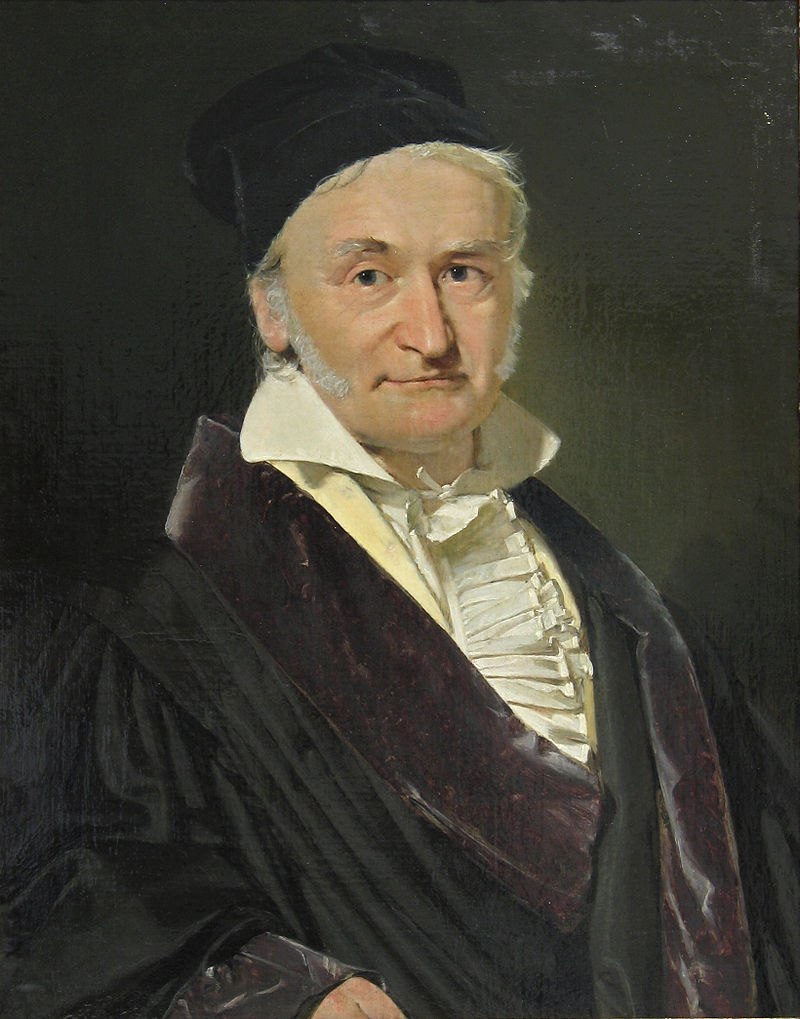
\includegraphics[width=0.4\textwidth]{imagenes/imagenes01/T01IM04.png}
	\end{figure}

Gauss fue un matemático, astrónomo, y físico alemán que contribuyó significativamente en muchos ámbitos, incluida la teoría de números, el análisis matemático, la geometría diferencial, la estadística, el álgebra, la geodesia, el magnetismo y la óptica. Considerado ya en vida como Princeps Mathematicorum, Gauss ha tenido una influencia notable en muchos campos de la matemática y de la ciencia.
\end{multicols}
Gauss pronto fue reconocido como un niño prodigio, pese a provenir de una familia campesina de padres con poca cultura: su madre sabía leer, aunque no escribir; su padre sí, pero en cuanto a las matemáticas, no pasaba de la aritmética más elemental. De Carl Friedrich Gauss existen muchas anécdotas acerca de su asombrosa precocidad. Hizo sus primeros grandes descubrimientos en el bachillerato, siendo a apenas un adolescente, y completó su magnum opus, Disquisitiones arithmeticae, a los veintiún años (1798), aunque se publicó en 1801. Fue un trabajo fundamental para consolidar la teoría de los números y ha moldeado esta área hasta los días presentes.

\end{myexampleblock}	
	

	
El método de Gauss para la solución de SEL es un método `muy robusto' y es aplicable a cualquier sistema independientemente de su número de ecuaciones o incógnitas. Es por ellos que se recomienda al lector/a que siga todos los ejercicios para asegurarse que entiende bien el método. En temas posteriores veremos otros métodos de resolución (Rouché, ecuaciones matriciales), que tendrán sus ventajas e inconvenientes respecto del método de Gauss pero no son tan potentes como éste.
 
Empezamos una colección de ejercicios resueltos en que se intentará que muestren explícitamente todos los pasos. El/la lector/a debe asegurarse que entiende bien todos los pasos y verse capaz de enfrentarse a los problemas propuestos con solución. Recuerda que cada problema es un mundo y solo al hacer muchos de ellos verás un abanico grande de posibilidades.

Los problemas de discusión de sistemas se dejan, como se ha mencionado anteriormente, para cuando se estudie el `teorema de Rocuché-Frobenius' que es una herramienta matemática más adecuada para estos menesteres.

También se incluyen, a modo de anécdota, algunos problemas de enunciado de los que hay que extraer el SEL correspondiente, resolver e interpretar la solución obtenida.
\subsection{Ejercicios resueltos}

Veamos un problema donde hay que intercambiar ecuaciones e incógnitas (avisando en este caso) para conseguir pivote $\pm 1$. Esto no es necesario, pero es conveniente para minimizar errores.

\begin{ejre} Resuelve: $\quad \begin{cases}2x+3y-4z=7\\3x+5y-z=6\\-3x+2y+5z=-3\end{cases}$ 
\end{ejre}
\begin{proofw}\renewcommand{\qedsymbol}{$\diamond$}
Matricialmente: $\quad \left[ \begin{matrix}
  2 & 3 & -4 \\ 3 & 5 & \boldsymbol{-1} \\ -3 & 2 & 5 
 \end{matrix}\right. 
 \left| \begin{matrix}
  7 \\ 6 \\ -3 
 \end{matrix}\right] \to$ 
\textcolor{gris}{$[E2 \leftrightarrow E1 ] \to (*)$}

Intercambiamos la ecuación 2 por la 1 y, luego, cambiamos de orden las incógnitas (*), para que el coeficiente $\boldsymbol{-1}$ aparezca en el lugar $1,1$ de la matriz y sea más sencillo combinar las otras ecuaciones con la primera para obtener ceros por debajo del $\boldsymbol{-1}$. Aunque no es necesario advertir del cambio de orden de las ecuaciones, sí lo es para el cambio de las incógnitas (lo hemos hecho añadiendo una fila a la matriz) ya que, de otro modo, pensaríamos que las incógnitas van en el orden habitual $x,y,z$.

$\left[ \begin{matrix}
  3 & 5 & \boldsymbol{-1} \\ 2 & 3 & -4 \\ -3 & 2 & 5 
 \end{matrix}\right. 
 \left| \begin{matrix}
  6 \\ 7 \\ -3  
 \end{matrix}\right] \to$
 $\left[ \begin{matrix}
  \boldsymbol{z} &  \boldsymbol{x} &  \boldsymbol{y} \\
  \boldsymbol{-1} & 3 & 5 \\ -4 & 2 & 3 \\ 5 & -3 & 2 
 \end{matrix}\right. 
 \left| \begin{matrix}
  \\ 6 \\ 7 \\ -3 
 \end{matrix}\right] \to$
 \textcolor{gris}{$\left[ \begin{matrix} E2 \to E2-4E1 \\ E3 \to E3+5E1 \end{matrix} \right] \to $}
 
 $\left[ \begin{matrix}
  z & x & y \\
 -1 & 3 & 5 \\ 0 & -10 & -17 \\ 0 & 12 & 27 
 \end{matrix}\right. 
 \left| \begin{matrix}
  \\ 6 \\ -17 \\ 27 
 \end{matrix}\right] \to$
 \textcolor{gris}{$[E3 \to 10E3-17E2] \to $}
 
  $\left[ \begin{matrix}
  z & x & \boldsymbol{y} \\
 -1 & 3 & 5 \\ 0 & -10 & -17 \\ 0 & 0 & 66 
 \end{matrix}\right. 
 \left| \begin{matrix}
  \\ 6 \\ -17 \\ 66 
 \end{matrix}\right] \to \begin{cases}
 \; \; 66y=66 \to \boldsymbol{y=1} \\
 \; -10x-17\cdot 1=-17 \to \boldsymbol{x=0}\\
 \; -z+3\cdot 0 + 5 \cdot 1 = 6 \to \boldsymbol{z=-1}	
 \end{cases}
$

Los transformaciones de Gauss escogidas para conseguir ceros no es necesario explicitarlas pero, de momento, lo haremos para dar más claridad al proceso.

!`Atención!: la última incógnita ahora es `$y$' no `$z$' como hemos indicado en la primera fila de la matriz. 

Despejando en cascada hemos encontrado	$\boldsymbol{x=0; \; y=1; \; z=-1}$, solución única: \textbf{SDC}.	
\end{proofw}

El método de Gauss no solo se aplica a `sistemas cuadrados', del mismo número de ecuaciones que de incógnitas si no que se puede aplicar en cualquier caso, con más ecuaciones que incógnitas o con más incógnitas que ecuaciones. En ambos casos el objetivo es el mismo, triangularizar la matriz, que por debajo de la diagonal todos los elementos sean ceros. Analizamos esto en los  siguientes ejercicios resueltos.
\begin{ejre} 
Resuelve: $\quad \left\{ \begin{matrix}
x&+2y&-5z&-t&+2u&=-3\\
&y&-2z&+t&-4u&=1\\
2x&-3y&+4z&+2t&-u&=9	
\end{matrix} \right.$
	
\end{ejre}
\begin{proofw}\renewcommand{\qedsymbol}{$\diamond$}

$\left[ \begin{matrix}
  1 & 2 & -5 & -1 & 2 \\ 0 & 1 & -2 & 1 & -4 \\ 2 & -3 & 4 & 2 & -1  
 \end{matrix}\right. 
 \left| \begin{matrix}
  -3 \\ 1 \\ 9 
 \end{matrix}\right] \to  $
$\left[ \begin{matrix}
  1 & 2 & -5 & -1 & 2 \\ 0 & 1 & -2 & 1 & -4 \\ 0 & -7 & 14 & 4 & -5  
 \end{matrix}\right. 
 \left| \begin{matrix}
  -3 \\ 1 \\ 15 
 \end{matrix}\right] \to  $
 
 \noindent \footnotesize{$\left[ \begin{matrix}
  1 & 2 & -5 & -1 & 2 \\ 0 & 1 & -2 & 1 & -4 \\ 0 & 0 & 0 & 11 & -33  
 \end{matrix}\right. 
 \left| \begin{matrix}
  -3 \\ 1 \\ 22 
 \end{matrix}\right] \to$}
 \scriptsize{$  \begin{cases}
  11t-33u=22; \; t-3u=2; u=\lambda \Rightarrow t=2+3\lambda \\
  y-2z+2+3\lambda-4\lambda=1; z=\mu \Rightarrow y=2\mu +\lambda -1\\
  x+2(2\mu+\lambda-1)-5\mu-2-3\lambda+2	\lambda=-3 \Rightarrow \\ \qquad  \qquad \qquad x=\mu-\lambda+1 \end{cases}$}\normalsize{.}



\noindent \small{$\boldsymbol {u=\lambda; \; t=2+3\lambda;\; z=\mu; \; y=2\mu+\lambda-1; \; x=\mu-\lambda+1\; \; \forall\; \lambda\; \mu \; \in \mathbb R }$}

Esta vez tenemos un \textbf{SCI}, doblemente indeterminado (hemos necesitado dos parámetros).
\end{proofw}


\begin{ejre} 
	Resuelve: $\quad \begin{cases}x+2y-3z=0\\-2x-z=-3\\-x+y=0\\-2y+4z=4\end{cases}$
\end{ejre}
\begin{proofw}\renewcommand{\qedsymbol}{$\diamond$}

$\left[ \begin{matrix}
  1 & 2 & -3 \\ -2 & 0 & -1 \\ -1 & 1 & 0 \\ 0 & -2 & 4  
 \end{matrix}\right. 
 \left| \begin{matrix}
  0 \\ -3 \\ 0 \\ 4
 \end{matrix}\right] \to $ 
 \textcolor{gris}{$\left[ \begin{matrix} E2 \to E2+2E1 \\ E3 \to E3+E1 \\ E4 \to E4\end{matrix} \right] \to $}
 $\left[ \begin{matrix}
  1 & 2 & -3 \\ 0 & 4 & -7 \\ 0 & 3 & -3 \\ 0 & -2 & 4  
 \end{matrix}\right. 
 \left| \begin{matrix}
  0 \\ -3 \\ 0 \\ 4
 \end{matrix}\right] \to $ 
 
 \noindent  \textcolor{gris}{$ \text{astucia:}\;  [E2 \leftrightarrow E3 ] \; \to $}
  $\left[ \begin{matrix}
  1 & 2 & -3 \\ 0 & 3 & -3 \\ 0 & 4 & -7 \\ 0 & -2 & 4  
 \end{matrix}\right. 
 \left| \begin{matrix}
  0 \\ 0 \\ -3 \\ 4
 \end{matrix}\right] \to $ \textcolor{gris}{$  \text{astucia:} \; [E2 \to E2/3]\; \to $}
 
 \noindent  $\left[ \begin{matrix}
  1 & 2 & -3 \\ 0 & 1 & -1 \\ 0 & 4 & -7 \\ 0 & -2 & 4  
 \end{matrix}\right. 
 \left| \begin{matrix}
  0 \\ 0 \\ -3 \\ 4
 \end{matrix}\right] \to $ \textcolor{gris}{$\left[ \begin{matrix}  E3 \to E3-4E2 \\ E4 \to E4+2E2 \end{matrix} \right] \to $}
 $\left[ \begin{matrix}
  1 & 2 & -3 \\ 0 & 1 & -1 \\ 0 & 0 & -3 \\ 0 & 0 & 42  
 \end{matrix}\right. 
 \left| \begin{matrix}
  0 \\ 0 \\ -3 \\ 4
 \end{matrix}\right] \to $ 
  
 \noindent \textcolor{gris}{$  \text{astucia:} \; [E3 \to E3/3]\; \to $}  $\left[ \begin{matrix}
  1 & 2 & -3 \\ 0 & 1 & -1 \\ 0 & 0 & -1 \\ 0 & 0 & 42  
 \end{matrix}\right. 
 \left| \begin{matrix}
  0 \\ 0 \\ -1 \\ 4
 \end{matrix}\right] \to $ \textcolor{gris}{$[E4 \to E4+42E3] \to $}
 
 \noindent  $\left[ \begin{matrix}
  1 & 2 & -3 \\ 0 & 1 & -1 \\ 0 & 0 & -1 \\ 0 & 0 & 0  
 \end{matrix}\right. 
 \left| \begin{matrix}
  0 \\ 0 \\ -1 \\ -38
 \end{matrix}\right] \to \; $ Última ecuación: $0=-38 \to \; $\textbf{SI}, el sistema no tiene solución.
\end{proofw}


\begin{ejre} 
Resuelve: $\quad \begin{cases}x-2y=0\\3x-y=5\\x-y=1\\x+y=3\\2x-3y=1\end{cases}$	
\end{ejre}
\begin{proofw}\renewcommand{\qedsymbol}{$\diamond$}

$\left[ \begin{matrix}
  1 & -2   \\ 3 & -1  \\ 1 & -1  \\ 1 & 1 \\ 2 & -3  
 \end{matrix}\right. 
 \left| \begin{matrix}
   0 \\ 5 \\ 1 \\ 3 \\ 1  
 \end{matrix}\right] \to \; $
 \textcolor{gris}{$\left[ \begin{matrix} E2 \to E2-3E1 \\ E3 \to E3-E1 \\ E4 \to E4-E1 \\ E5 \to E5-2E1   \end{matrix} \right] \to $} 
$\left[ \begin{matrix}
  1 & -2   \\ 0 & 5  \\ 0 & 1  \\ 0 & 3 \\ 0 & 1  
 \end{matrix}\right. 
 \left| \begin{matrix}
   0 \\ 5 \\ 1 \\ 3 \\ 1  
 \end{matrix}\right] \to \; $
 \textcolor{gris}{$  \text{astucia:} \; [E3 \leftrightarrow E2 ]\; \to $} 
 
 \noindent $\left[ \begin{matrix}
  1 & -2   \\ 0 & 1  \\ 0 & 5  \\ 0 & 3 \\ 0 & 1  
 \end{matrix}\right. 
 \left| \begin{matrix}
   0 \\ 1 \\ 5 \\ 3 \\ 1  
 \end{matrix}\right] \to \; $
 \textcolor{gris}{$\left[ \begin{matrix} E3\to E3-5E2 \\ E4\to E4-3E2 \\ E5 \to E5-E2  \end{matrix} \right] \to $}
 $\left[ \begin{matrix}
  1 & -2   \\ 0 & 1  \\ \text{\textst{ 0 }}  & \text{\textst{ 0 }}   \\ \text{\textst{ 0 }}  & \text{\textst{ 0 }}  \\ \text{\textst{ 0 }}  & \text{\textst{ 0 }}   
 \end{matrix}\right. 
 \left| \begin{matrix}
   0 \\ 1 \\ \text{\textst{ 0 }}  \\ \text{\textst{ 0 }}  \\ \text{\textst{ 0 }}   
 \end{matrix}\right] \to \; $ 
 
 Última ecuación (eliminadas las trivialidades): $\; \boldsymbol{y=1} \Rightarrow x-2=0 \to \boldsymbol{x=2}$

Tenemos un \textbf{SCD} cuya solución única es $\boldsymbol{x=2; \; y=1}$, que muchos autores pueden representar como $(2,1)$.
\end{proofw}


\begin{ejre} 
Resuelve: $ \quad \begin{cases}-x+y-z=-2\\x-y+2z=4\\x+z+t=3\\x+2z+t=1 \end{cases}$
\end{ejre}
\begin{proofw}\renewcommand{\qedsymbol}{$\diamond$}

$\left[ \begin{matrix}
 -1 & 1 & -1 & 0\\ 1 & -1 & 2 & 0 \\ 1 & 0 & 1 & 1 \\ 1 & 0 & 2 & 1 
 \end{matrix}\right. 
 \left| \begin{matrix}
  -2 \\ 4 \\ 3  \\ 1
 \end{matrix}\right] \to$
\textcolor{gris}{$\begin{cases} E2 \to E2+E1 \\ E3 \to E3+E1 \\ E4 \to E4+E1 \end{cases} \to $}
$\left[ \begin{matrix}
 1 & 1 & -1 & 0\\ 0 & 0 & 1 & 0 \\ 0 & 1 & 0 & 1 \\ 0 & 1 & 1 & 1 
 \end{matrix}\right. 
 \left| \begin{matrix}
  -2 \\ 2 \\ 1  \\ -1
 \end{matrix}\right] \to$
 
Intercambiamos las ecuaciones 2 y 3: \textcolor{gris}{$[\;E2 \leftrightarrow E3 \; ]$}

\noindent $\left[ \begin{matrix}
 1 & 1 & -1 & 0\\ 0 & 1 & 0 & 1 \\ 0 & 0 & 1 & 0 \\ 0 & 1 & 1 & 1 
 \end{matrix}\right. 
 \left| \begin{matrix}
  -2 \\ 1 \\ 2  \\ -1
 \end{matrix}\right] \to$ \textcolor{gris}{$\begin{cases} E3 \to E3 \\ E4 \to E4-E2 \end{cases} \to $}
 $\left[ \begin{matrix}
 1 & 1 & -1 & 0\\ 0 & 1 & 0 & 1 \\ 0 & 0 & 1 & 0 \\ 0 & 0 & 1 & 0 
 \end{matrix}\right. 
 \left| \begin{matrix}
  -2 \\ 1 \\ 2  \\ -2
 \end{matrix}\right] \to$
 


\noindent  \textcolor{gris}{$[\;E4 \to E4-E3 \;] \to $} $\left[ \begin{matrix}
 1 & 1 & -1 & 0\\ 0 & 1 & 0 & 1 \\ 0 & 0 & 1 & 0 \\ 0 & 0 & 0 & 0 
 \end{matrix}\right. 
 \left| \begin{matrix}
  -2 \\ 1 \\ 2  \\ -4
 \end{matrix}\right] \to$ Última ecuación: $0=-4$, hemos llegado a una incompatibilidad, tenemos pues un \textbf{SI}
\end{proofw}

\begin{ejre} 
Resuelve: $\; \begin{cases} 2x+3y+4z+5t=0\\-3x-2y+3z-2t=-2\\4x+5y-2z+2t=7  \end{cases}\; $  \footnotesize{\textcolor{gris}{sin ningún pivotes $\pm 1$}}\normalsize{.}
\end{ejre}
\begin{proofw}\renewcommand{\qedsymbol}{$\diamond$}

$\left[ \begin{matrix}
  2 & 3 & 4 & 5 \\ -3 & -2 & 3 & -2 \\ 4 & 5 & -2 & 2 
 \end{matrix}\right. 
 \left| \begin{matrix}
  9 \\ -2 \\ 7 
 \end{matrix}\right] \to $
 \textcolor{gris}{$\begin{cases} E2\to 2E2+3E1 \\ E3 \to E3-2E1  \end{cases} \to $}
$\left[ \begin{matrix}
  2 & 3 & 4 & 5 \\ 0 & 5 & 18 & 11 \\ 0 & -1 & -10 & -8 
 \end{matrix}\right. 
 \left| \begin{matrix}
  9 \\ 23 \\ -11 
 \end{matrix}\right] \to $
 
\noindent \textcolor{gris}{$[\; E3 \to 5E3+E2 \; ] \to $}
$\left[ \begin{matrix}
  2 & 3 & 4 & 5 \\ 0 & 5 & 18 & 11 \\ 0 & 0 & 32 & 29 
 \end{matrix}\right. 
 \left| \begin{matrix}
  9 \\ 23 \\ 32 
 \end{matrix}\right] \to 32z+29t=32; \; \boldsymbol{t=\lambda, \; \forall \lambda \in \mathbb R}$
 
 \noindent $\boldsymbol{z=1-\frac{29}{32}\lambda}; \; \to 5y+18(1-\frac{29}{32}\lambda)+11 \lambda =23 \to \boldsymbol{y=1-\frac {371}{80}\lambda}\; \to 2x+3(1-\frac {371}{80}\lambda)+4(1-\frac{29}{32}\lambda)+5\lambda = 9 \to \boldsymbol{x=1-\frac{1003}{160}\lambda}\; $. \textbf{SCI}.
\end{proofw}

\begin{ejre} 
Resuelve: $\quad \begin{cases} 5x-3y+4z=0\\2x+5y-z=0\\-3x-2y+6z=0   \end{cases}$ 
\end{ejre}
\begin{proofw}\renewcommand{\qedsymbol}{$\diamond$}
\small{$\left[ \begin{matrix}
  5 & -3 & 4 \\ 2 & 5 & -1 \\ -3 & -2 & 6 
 \end{matrix}\right. 
 \left| \begin{matrix}
  0 \\ 0 \\ 0 
 \end{matrix}\right] \to $}
\small{\textcolor{gris}{$E2\leftrightarrow E1 \to $}}
 $\left[ \begin{matrix}
   2 & 5 & -1  \\ 5 & -3 & 4 \\ -3 & -2 & 6 
 \end{matrix}\right. 
 \left| \begin{matrix}
  0 \\ 0 \\ 0 
 \end{matrix}\right]  \to $
 \footnotesize{\textcolor{gris}{Intercambio $x\leftrightarrow z \to$}}
 
\normalsize{ \noindent  $\left[ \begin{matrix}
  \boldsymbol{z} & \boldsymbol{y} & \boldsymbol{x} \\
   -1 & 5 & 2  \\ 4 & -3 & 5 \\ 6 & -2 & -3 
 \end{matrix}\right. 
 \left| \begin{matrix}
 \\ 0 \\ 0 \\ 0 
 \end{matrix}\right]  \to $
 \textcolor{gris}{$\begin{cases} E2\to E2+4E1 \\ E3 \to E3+6E1 \end{cases} \to $}
  $\left[ \begin{matrix}
  \boldsymbol{z} & \boldsymbol{y} & \boldsymbol{x} \\
   -1 & 5 & 2  \\ 0 & 17 & 13 \\ 0 & 28 & 11 
 \end{matrix}\right. 
 \left| \begin{matrix}
 \\ 0 \\ 0 \\ 0 
 \end{matrix}\right]  \to $}
 
 \noindent \textcolor{gris}{$[E3 \to 17E3-28E2]\to $}
   $\left[ \begin{matrix}
  \boldsymbol{z} & \boldsymbol{y} & \boldsymbol{x} \\
   -1 & 5 & 2  \\ 0 & 17 & 13 \\ 0 & 0 & -183 
 \end{matrix}\right. 
 \left| \begin{matrix}
 \\ 0 \\ 0 \\ 0 
 \end{matrix}\right]  \to -183x=0 \Rightarrow \boldsymbol{x=y=z=0}\; $ \normalsize{SCD y homogéneo, solo tiene la solución trivial.}

\end{proofw}

\begin{ejre} 
Resuelve: $\quad \begin{cases} x+2y-3z=0\\2x+y-z=0\\x-y+2z=0  \end{cases}$ 
\end{ejre}
\begin{proofw}\renewcommand{\qedsymbol}{$\diamond$}
$\left[ \begin{matrix}
  1 & 2 & -3 \\ 2 & 1 & -1 \\ 1 & -1 & 2 
 \end{matrix}\right. 
 \left| \begin{matrix}
  0 \\ 0 \\ 0 
 \end{matrix}\right] \to $
 \textcolor{gris}{$\begin{cases} E2 \to E2-2E1 \\ E3 \to E3-E1  \end{cases} \to $}
 $\left[ \begin{matrix}
  1 & 2 & -3 \\ 0 & -3 & 5 \\ 0 & -3 & 5 
 \end{matrix}\right. 
 \left| \begin{matrix}
  0 \\ 0 \\ 0 
 \end{matrix}\right] \to $
 
 \noindent \textcolor{gris}{$[ E3 \to E3-E2] \to$}
  $\left[ \begin{matrix}
  1 & 2 & -3 \\ 0 & -3 & 5 \\ \text{\textst{ 0 }} 
 & \text{\textst{ 0 }} 
 & \text{\textst{ 0 }} 
 
 \end{matrix}\right. 
 \left| \begin{matrix}
  0 \\ 0 \\ \text{\textst{ 0 }} 
 \end{matrix}\right] \to $ Eliminando la trivialidad, la última ecuación dice: $-3y+5z=0 \to \boldsymbol{z=\lambda , \; \forall \lambda \in \mathbb R} ;\; \boldsymbol{y=\frac 5 3 \lambda}; \; \; x+2 \frac 5 3 \lambda -3\lambda =0 \to \bold{x=-\frac 1 3 \lambda} $. Tenemos un \textbf{SCI}, como es homogéneos debe contener a la solución trivial. Basta, para ello, tomar $\lambda=0$.
\end{proofw}

\begin{ejre} 
Resuelve: $\begin{cases} x+y+z+t&=0\\x-2y+3z&=0\\2x-y+4z+t&=0 \end{cases}$
\end{ejre}
\begin{proofw}\renewcommand{\qedsymbol}{$\diamond$}
$\left[ \begin{matrix}
  1 & 1 & 1 & 1 \\ 1 & -2 & 3 & 0\\ 2 & -1 & 4 & 1 
 \end{matrix}\right. 
 \left| \begin{matrix}
  0 \\ 0 \\ 0 
 \end{matrix}\right] \to$
 \textcolor{gris}{$\begin{cases} E2\to E2-E1\\E3\to E3-2E1 \end{cases} \to  $}
$\left[ \begin{matrix}
  1 & 1 & 1 & 1 \\ 0 & -3 & 2 & -1\\ 0 & -3 & 2 & -1 
 \end{matrix}\right. 
 \left| \begin{matrix}
  0 \\ 0 \\ 0 
 \end{matrix}\right] \to$
 	
\noindent \textcolor{gris}{$[E3 \to E3-E2] \to $}
$\left[ \begin{matrix}
  1 & 1 & 1 & 1 \\ 0 & -3 & 2 & -1\\ \text{\textst{ 0 }} & \text{\textst{ 0 }} & \text{\textst{ 0 }} & \text{\textst{ 0 }} 
 \end{matrix}\right. 
 \left| \begin{matrix}
  0 \\ 0 \\ \text{\textst{ 0 }} 
 \end{matrix}\right] \to$ última ecuación:
 
 \noindent $-3y+2z-t=0; \boldsymbol{y=\lambda ;\;  z=\mu; \; \forall \lambda, \mu \; \in \mathbb R}\to \boldsymbol{t=-3\lambda+2\mu} \to x+\lambda+\mu+(-3\lambda+2\mu)=0 \to \bold{x=2\lambda-3\mu}; \; SCI$

\end{proofw}


\begin{ejre} 
Como se comenta al principio de la sección ejercicios, el método de Gauss-Jordan es una ampliación del método de Gauss que consiste en, una vez triangularizada inferiormente la matriz asociada al SEL (ceros por debajo de la diagonal), hacerlo ahora por arriba. De este modo queda una matriz `diagonalizada' en la que de cada fila se despeja cada incógnita.

\noindent Resuelve, por el método de Gauss- Jordan el SEL : $\begin{cases}  x+2y-z&=-2 \\ x+z&=2 \\ 2x-y+2z&=5\end{cases}$
\end{ejre}
\begin{proofw}\renewcommand{\qedsymbol}{$\diamond$}

$\left[ \begin{matrix}
  1 & 2 & -1 \\ 1 & 0 & 1 \\ 2 & -1 & 2 
 \end{matrix}\right. 
 \left| \begin{matrix}
  -2 \\ 2 \\ 5  
 \end{matrix}\right] \to  $
 \textcolor{gris}{$\begin{cases}E2 \to E2-E1 \\ E3 \to E3-2 E1 \end{cases} $}
 $ \to \left[ \begin{matrix}
  1 & 2 & -1 \\ 0 & -2 & 2 \\ 0 & -5 & 4 
 \end{matrix}\right. 
 \left| \begin{matrix}
  -2 \\ 4 \\ 9  
 \end{matrix}\right] \to$
 
 \noindent \textcolor{gris}{$[E2 \leftrightarrow E2/2 ] $}
 $ \to \left[ \begin{matrix}
  1 & 2 & -1 \\ 0 & -1 & 1 \\ 0 & -5 & 4 
 \end{matrix}\right. 
 \left| \begin{matrix}
  -2 \\ 2 \\ 9  
 \end{matrix}\right] \to$
  \noindent \textcolor{gris}{$[E3 \leftrightarrow E3-5E1 ] $}
  $ \to \left[ \begin{matrix}
  1 & \boxed{2} & \boxed{-1} \\ 0 & -1 & \boxed{1} \\ 0 & 0 & -1 
 \end{matrix}\right. 
 \left| \begin{matrix}
  -2 \\ 2 \\ -1  
 \end{matrix}\right] \to$
  \textcolor{gris}{Ahora, al revés: $\begin{cases}E2 \to E2+E3 \\ E1 \to E1-E3 \end{cases} $}
   $ \to \left[ \begin{matrix}
  -1 & \boxed{-2} & 0 \\ 0 & -1 & 0 \\ 0 & 0 & -1 
 \end{matrix}\right. 
 \left| \begin{matrix}
  1 \\ 1 \\ -1  
 \end{matrix}\right] \to$
 \textcolor{gris}{$\left[\begin{matrix}E3\to \\ E3-E2\end{matrix} \right]$}
 
 \noindent    $ \to \left[ \begin{matrix}
  -1 & 0 & 0 \\ 0 & -1 & 0 \\ 0 & 0 & -1 
 \end{matrix}\right. 
 \left| \begin{matrix}
  -1 \\ 1 \\ -1  
 \end{matrix}\right] \to \begin{matrix} \text{ matriz } \\ \text{diagonalizada}  \end{matrix} \to \begin{cases} \; -x=-1 \to \boldsymbol{x=1} \\ \; -y=1 \to \boldsymbol{y=-1} \\ \; -z=-1 \to \boldsymbol{z=1}   \end{cases}\; \; \boldsymbol{SCD}$
\end{proofw}

\begin{ejre} 
Encuentra una solución, si es posible, del siguiente sistema en que $z=3$. ?`Existe alguna solución en que $x=2$?

$\begin{cases} x-y+z=1\\x+y-z=1\\5x+y-z=5  \end{cases}$
\end{ejre}
\begin{proofw}\renewcommand{\qedsymbol}{$\diamond$}
Apliquemos el método de Gauss para resolver el sistema y encontrar todas sus soluciones y luego ya intentaremos contestar a las preguntas que nos formulan.

$\left[ \begin{matrix}
  1 & -1 & 1 \\ 1 & 1 & -1 \\ 5 & 1 & -1 
 \end{matrix}\right. 
 \left| \begin{matrix}
  1 \\ 1 \\ 5 
 \end{matrix}\right] \to $
 $\left[ \begin{matrix}
  1 & -1 & 1 \\ 0 & 2 & -2 \\ 0 & 6 & -6 
 \end{matrix}\right. 
 \left| \begin{matrix}
  1 \\ 0 \\ 0 
 \end{matrix}\right] \to $
  $\left[ \begin{matrix}
  1 & -1 & 1 \\ 0 & 2 & -2 \\ \text{\textst{ 0 }} & \text{\textst{ 0 }} & \text{\textst{ 0 }} 
 \end{matrix}\right. 
 \left| \begin{matrix}
  1 \\ 0 \\ \text{\textst{ 0 }}
 \end{matrix}\right] \to $
 
 $2y-2z=0; \; \boldsymbol{z=\lambda}, \; ºforall \lambda \in \mathbb R \to -\lambda+\lambda=1 \to \boldsymbol{x=1}$
 
 Tenemos un $\textbf{SCI}, \text{ con soluciones : } x=1; \; y=\lambda; \; z=\lambda; \quad \forall \lambda \in \mathbb R$. Respondamos ahora a las preguntas del problema:
 
--- Encuentra una solución, si es posible, del siguiente sistema en que $z=3 \Rightarrow $ \textbf{Sí}, ya que si $z=3=\lambda \to y=3; \; x=1$
 
 --- ?`Existe alguna solución en que $x=2$? \textbf{No}, necesariamente, en todas las soluciones $x=1$
 
\end{proofw}

\begin{ejre} 
En ocasiones, ante la sencillez del problema, no es necesario seguir todos los pasos.

Resuelve: 

$a) \quad \begin{cases} 2x-3z&=2\\2x+3y-4z&=-1\\z&=0 \end{cases} \qquad \qquad b) \quad \begin{cases} y+z&=4\\x-3y+2z&=7\\y-z&=2 \end{cases}$
\end{ejre}
\begin{proofw}\renewcommand{\qedsymbol}{$\diamond$}
a) En este caso, usando un poco la astucia no hace falta hacer nada (colocamos $z$ como primera incógnita, luego $x$ e $y$ por último. Escribimos como primera ecuación la tercera, como segunda la primera y como tercera la segunda y ya tenemos el sistema escalonado). 

Última ecuación $\boldsymbol{z=0}$, yendo a la primera ecuación: $2x-3\cdot0=2 \to \boldsymbol{x=1}$ y, finalmente, acudiendo a la segunda ecuación: $2\cdot 1 +3y-4\cdot 0=-1 \to \boldsymbol{y=-1}$, Tenemos un \textbf{SDC}.

b) Las ecuaciones uno y tres se resuelven inmediatamente sin más que sumarlas, $2y=6 \to \boldsymbol{y=3}$; sustituyendo en la primera, $3+z=4 \to \boldsymbol{z=1}$ y, finalmente, acudiendo a la segunda ecuación: $x-3\cdot 3 +2\cdot 2=7 \to \boldsymbol{x=14}$. Se trata de un \textbf{SCD}.
\end{proofw}


\begin{ejre} 
Un automóvil sube las cuestas a $54\; km/h$, las baja a $90\; km/h$ y en llano circula a $80\;  km/h$. Para ir de $A$ a $B$ tarda $2$ horas y 30 minutos, y para volver de $B$ a $A$, 2 horas y 45 minutos. ¿Cuál es la longitud de camino llano entre $A$ y $B$ si sabemos que la distancia entre $A$ y $B$ es de $192\;  km$? 
\end{ejre}
\begin{proofw}\renewcommand{\qedsymbol}{$\diamond$}
\begin{figure}[H]
		\centering
		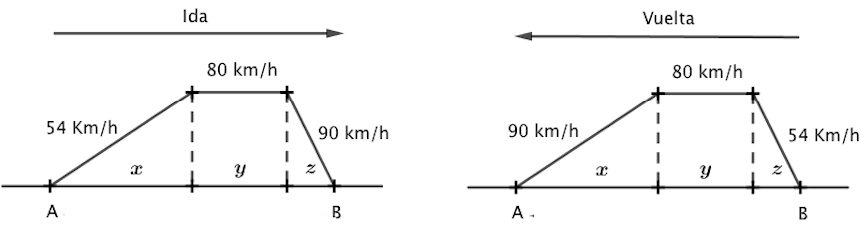
\includegraphics[width=.9\textwidth]{imagenes/imagenes01/T01IM06.png}
	\end{figure}

\vspace{-2mm}	

	Suponiendo que el vehículo viaja a $v$ constante: $v=\frac s t \to t=\frac s v$. A la ida $t_{ida}=t_{x,s}+t_{y,n}+t_{z,b}$, a la vuelta $t_{vuelta}=t_{x,b}+t_{y,n}+t_{z,s}$, donde los subíndices $\; x,y,z\; $ indican los tramos que circula el coche a distintas velocidades y $\; s,n,b\; $ indican los tramos de `subida', `normal' y `bajada', respectivamente.
	
	La traducción del enunciado al leguaje algebraico conduce al sistema:
	
	$\begin{cases} x+y+z&=192\\ \frac{x}{54} + \frac{y}{80}+\frac{z}{90}&=2.5 \\ \frac{x}{90}+\frac{y}{80}+\frac{z}{94}&=2.75   \end{cases} \; \; $
	Lo más cómodo es multiplicar las ecuaciones 2 y 3 por el mcm de los denominadores (2160, en este caso) y conseguir un sistema sin denominadores que, resolviendo por Gauss tiene por solución única (\textbf{SCD}):
	
	$\boldsymbol{x=31.725 \; km; \; y= 94.800 \; km; \; z= 65.465 \; km}$, con lo que \textbf{la longitud de camino llano es de} $\boldsymbol{94.8 \; km}$.
\end{proofw}


\begin{ejre} 
Un cajero automático contiene $95$ billetes de $10$, $20$ y $m$ euros. Se sabe que tiene almacenados $2000$ euros y que el número de billetes de $10$ euros es el doble que el número de billetes de $20$ euros. 

\begin{enumerate}[a) ]
\item Plantea un sistema de ecuaciones que refleje las condiciones del problema. ?`Qué valores puede tomar $m$?
\item Resuelve el sistema para $m=5$ y para  $m = 50$. 
\end{enumerate} 
\end{ejre}
\begin{proofw}\renewcommand{\qedsymbol}{$\diamond$}
Planteemos y resolvamos el problema y, después, contestaremos a las preguntas que se formulan.

Llamamos $x$ al número de billetes de $10$ euros, $y$ al número de billetes de $20$ euros y $z$ al número de billetes de $m$ euros. Con esto, el sistema es:

\noindent $\begin{cases}x+y+z=95\\10x+20y+mz=2000\\x=2y  \end{cases}$. Sistema que hay que preparar antes de aplicar el método de Gauus pasando todas las incógnitas a la izquierda y los términos independientes a la derecha. Aprovechamos para escribir la segunda ecuación en último lugar y usar el parámetro $m$ lo más tarde posible. Ya advertimos que para discutir sistemas veremos métodos mejores que Gauss, pero en este caso vamos a resolverlo.

\noindent $\begin{cases}x+y+z=95 \\x-2y=0 \\10x+20y+mz=2000  \end{cases} \to $
$\left[ \begin{matrix}
  1 & 1 & 1 \\ 1 & -2 & 0 \\ 10 & 20 & m 
 \end{matrix}\right. 
 \left| \begin{matrix}
  95 \\ 0 \\ 2000 
 \end{matrix}\right] \to $
\textcolor{gris}{ $ \begin{cases} E2 \to E2-E1 \\ E3 \to E3-10E1 \end{cases} \to $}

\noindent $\left[ \begin{matrix}
  1 & 1 & 1 \\ 0 & -3 & -1 \\ 0 & 10 & m-10 
 \end{matrix}\right. 
 \left| \begin{matrix}
  95 \\ -95 \\ 1050 
 \end{matrix}\right] \to $
 \textcolor{gris}{$[E3 \to 3E3+10E2] \to $}
  $\left[ \begin{matrix}
  1 & 1 & 1 \\ 0 & -3 & -1 \\ 0 & 0 & 3m-40 
 \end{matrix}\right. 
 \left| \begin{matrix}
  95 \\ -95 \\ 2200
 \end{matrix}\right]  $
 
 Última ecuación: $(3m-40)z=2200$, el sistema es incompatible si $3m-40=0\to m=40/3 \notin \mathbb N$, como $m$ hace referencia a billetes de determinada cantidad, $m \in \{5,10,20,100, 200, 500\}$, luego es sistema es siempre \textbf{SCD} para los posibles valores de $m$.
 
 Aunque el enunciado pide analizar los casos $m=5$ y $m=50$, vamos a estudiar todas las posibilidades:
 
\noindent  --- $m=5 \to (3m-40)z=(15-40)z=2200\to z<0$, no tiene sentido una cantidad de billetes negativa.  No hay solución.
 
\noindent  --- $m=10 \to (3m-40)z=(10-40)z=-10z=2200\to z<0$, no tiene sentido una cantidad de billetes negativa.  No hay solución.
 
  
\noindent  --- $m=50 \to (3m-40)z=(150-40)z=110z=2200\to z=20; \; 3y+20=95\to y=25; \; x+25+20=95 \to x=50$, la solución es \textbf{50 billetes de 1o euros, 25 de 20 euros y 20 de 50 euros.}
 
\noindent  --- $m=100 \to (3m-40)z=(300-40)z=260z=2200 \to z=8.46\cdots \notin \mathbb N$. No hay solución.
 
 \noindent  --- $m=200 \to (3m-40)z=(600-40)z=560z=2200 \to z=3.92\cdots \notin \mathbb N$. No hay solución.
  
\noindent  --- $m=500 \to (3m-40)z=(1500-40)z=1460z=2200 \to z=1.50\cdots \notin \mathbb N$. No hay solución.
\end{proofw}

\begin{ejre}
	Razona si los siguientes sistemas son equivalentes o no: $\quad \begin{cases}x-3y+4z&=7\\3x+2z&=0 \end{cases} \qquad \qquad \qquad  \begin{cases}x=-2\\y=1\\z=3 \end{cases}$
	
	\noindent ?`Puedes añadir una ecuación al primer sistema para que resulte incompatible?
\end{ejre}
\begin{proofw}\renewcommand{\qedsymbol}{$\diamond$}
	El segundo sistema es SCD, su única solución es $(-2,1,3)$, que también es solución del primer sistema. Pero éste tiene infinitas soluciones puesto que se trata de un sistema con más incógnitas que ecuaciones que admite, al menos, una solución (no es SI). El primer sistema es pues SCI, por lo que los dos sistemas \textbf{no son equivalentes}.
	
	Para añadir una ecuación más al primer sistema y que resulte incompatible la ecuación añadida debe ser de la forma: $a(x-3y+4z)+b(3x+2z)\neq a\cdot 7+b \cdot 0$, Por ejemplo, con $a=b=1$, si se añade la ecuación $(x-3y+4z)+(3x+2z)=1 \rightarrow \boldsymbol{4x-3y+6z=1}$, tendremos un SI
\end{proofw}

\begin{ejre}
Considera el SEL: $\begin{cases} 2x-y+z=5 \\ -x+2y=3  \end{cases}$.

Añade, si es posible, una nueva ecuación al sistema para que resulte:  a) Incompatible, b) Compatible indeterminado, c) Compatible determinado. Justifica tus respuestas.
\end{ejre}
\begin{proofw}\renewcommand{\qedsymbol}{$\diamond$}
	Añadir una ecuación para que se produzca incompatibilidad consiste en añadir una contradicción, por ejemplo, si la primera ecuación da 5 y la segunda 3, la suma no puede ser nada que no sea 8. Por otra parte, añadir una ecuación para que el sistema sea compatible indeterminado consiste en añadir una trivialidad, algo que no aporte ninguna nueva información al sistema, por ejemplo, ecuación1 + ecuación 2 = 5+3=0. El sistema será compatible si hay solución única. Por ejemplo, dando un valor a $x$, de la segunda ecuación obtenemos la $y$ y despejamos en la primera. Sería suficiente con añadir una tercera ecuación de la forma $x=k$.
	
	--- SI: $a(2x-y+z)+b(-x+2y)\neq 5a+3b \to (a=b=1) \Rightarrow \boldsymbol{x+y+z=5}$
	
	--- SCI:  $a(2x-y+z)+b(-x+2y)= 5a+3b \to (a=b=1) \Rightarrow \boldsymbol{x+y+z=8}$
	
	---SCD: $\boldsymbol{x=1}$
\end{proofw}

\begin{ejre}
	Pon un ejemplo, cuando sea posible de un sistema de dos ecuaciones con tres incógnitas que sea: a) compatible determinado; b) compatible indeterminado; c) incompatible.
\end{ejre}
\begin{proofw}\renewcommand{\qedsymbol}{$\diamond$}
	
	\noindent a) Un sistema con menos ecuaciones que incógnitas jamás puede ser compatible determinado, con solo dos datos no podemos determinar tres valores (incógnitas).
	
	\noindent b) Un ejemplo sencillo es el siguiente sistema: $\begin{cases} x=1 \\y+z=1 \end{cases}$, de soluciones $(1,-\lambda,\lambda)$
	
	\noindent c) Un sistema incompatible con dos ecuaciones es que entren en contradicción. por ejemplo: $\begin{cases}x+y+z=1\\x+y+z=0\end{cases}$
\end{proofw}


\subsection{Ejercicios propuestos}
	\begin{figure}[H]
		\centering
		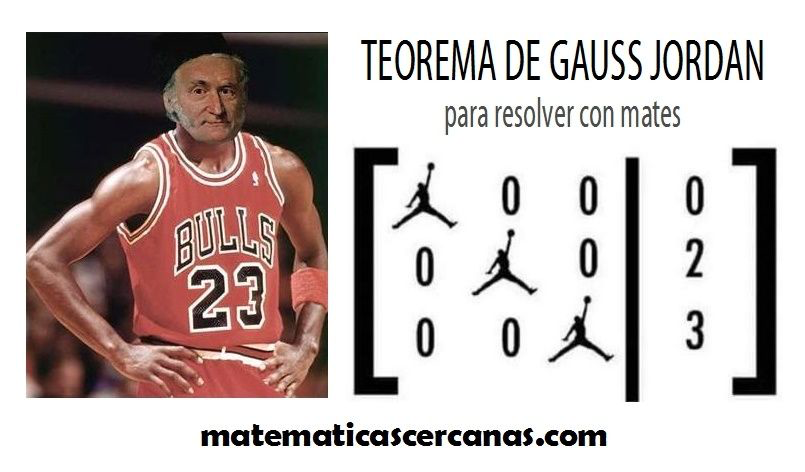
\includegraphics[width=0.8\textwidth]{imagenes/imagenes01/T01IM03.png}
	\end{figure}

\begin{enumerate}
\item $a) \quad \begin{cases}2x+6y+7z&=7\\x+2y-z&=-1\\5x+7y-4z&=9  \end{cases}\qquad b) \quad \begin{cases} x+y+z&=0\\x+2y+3z&=0\\3x+5y+7z&=1 \end{cases}$

\rightline{\textcolor{gris}{Solución: $a) \quad (10,-3,5); \; SCD; \qquad b) \quad SI$   }}

\item $a) \quad \begin{cases} 2x-y&=0\\-x+2y-z&=0\\-y+2z-t&=0\\-z+2t&=5 \end{cases} \qquad b) \quad \begin{cases} x+y-z&=2\\3x+3y+z&=2\\x+z=0\end{cases}$

\rightline{\textcolor{gris}{Solución: $a) \quad (1,2,3,4); \; SCD \qquad b) \quad (1,0,-1);\; SCD $ }}

\item $\qquad \begin{cases} x+y-3z-u&=-3\\x-y+2z-t&=-1\\4x-2y+6z+3t-4u&=3\\2x+4y-2z+4t-7u&=4 \end{cases}$

\rightline{\textcolor{gris}{Solución: $\left(\frac{7\lambda-2\mu-7}{2},\frac{5\lambda+2\mu-5}{2},\mu,3\lambda-3,\lambda \right)$  }}

\item $a) \quad \begin{cases} 3x-2y&=5\\x+4y&=4\\-x-2y&=-3  \end{cases}\qquad b) \quad \begin{cases} x+2z&=3\\x+y=2 \end{cases}$

\rightline{\textcolor{gris}{Solución: $a)\quad (2,1/2); \; SCD \qquad b) \quad (\lambda, 2-\lambda, (3-\lambda)/2); \; SCI$  }}

\item $a) \quad \begin{cases} -x+3y-z&=4\\x+4y&=5\\2x-6y+2z&=3  \end{cases}  \qquad b) \quad \begin{cases} 2x-y+z&=3\\x+2y-z&=4\\x-8y+5z&=-6 \end{cases}$

\rightline{\textcolor{gris}{Solución: $a)\quad SI; \qquad b) \quad (2-\lambda/5, 1+3\lambda/5,\lambda); \; SCI$  }}

\item $a) \quad \begin{cases} 3x-z&=4\\y+3x&=2 \end{cases} \qquad b) \quad \begin{cases} x+y+z&=1\\2x-3z&=5\\2y+5z&=2 \end{cases}$

\rightline{\textcolor{gris}{Solución: $a) \quad \left (\frac {4+\lambda} {3},2-3\lambda, \lambda \right) ; \; SCI \qquad b) \quad SI$  }}

\item $a) \quad \begin{cases} -3x+y+z&=1\\x-2y+z&=4\\-x+y-3z&=-7 \end{cases} \qquad b) \quad \begin{cases}2x-y+z&=3\\3x+y-z&=-3\\x-3y+3z&=9\\2x+4y-4z&=-12  \end{cases}$ 

\rightline{\textcolor{gris}{Solución: $a) \quad (0,1,-2); \; SCD \qquad b) \quad (2, \lambda -3, \lambda) \; \; SCI$ }}



\item $a) \quad \begin{cases}  x-y+z+t &= 0\\x+y+z-t &= 2\\x-y-z+t &= 2 \end{cases} \qquad b) \quad \begin{cases} 5x-y+3z &= -6\\x+3y-z &= 10\\2x-y+4z & =-2 \end{cases}$

\rightline{\textcolor{gris}{Solución: $a) \quad (2, 1+\lambda, -1, \lambda); \; SCI \qquad b) \quad (-1,4,1)$  }}

\item $a) \quad \begin{cases} 2x-y+z &= 5 \\ 3x+2y &= 1 \\ -x+4y-2z &= -9 \\ 6x+11y-3z &= -11  \end{cases} \qquad b) \quad \begin{cases} x+2y+z+t&=3\\-x+y+2t&=-1\\-x+7y+2z+8t&=1 \end{cases}$

\rightline{\textcolor{gris}{Solución: $a) \quad \left(\frac{11-2\lambda}{7}, \frac {-13+3\lambda}{7}, \lambda \right); \; SCI \qquad b) \quad SI$  }}

\item $a) \quad \begin{cases} 3x-5y+z&=0\\x-2y+z&=0\\x+y&=0 \end{cases} \qquad b) \quad \begin{cases} x-y-z&=0\\x+y+3z&=0\\x-5y-9z&=0 \end{cases}$

\rightline{\textcolor{gris}{Solución: $a) \quad (0,0,0)\; SCD \qquad b) \quad (-\lambda, -2\lambda, \lambda); \; SCI$  }}

\item $a) \quad \begin{cases} x+11y-4z&=0\\-2x+4y+z&=0\\ x+y-2z&=0\\2x-16y+5z&=0 \end{cases} \qquad b) \quad \begin{cases}   x+y+5z&=0\\3x-y-2t&=0\\x-y+z-t&=0\end{cases}$

\rightline{\textcolor{gris}{Solución: $a) \quad (0,0,0)\; SCD \qquad b) \quad (\lambda, -\lambda, 0, 2\lambda)\; \; SCI$  }}

\item $a) \quad \begin{cases} x-2y+3z&=0\\y+z&=0\\x-3y+2z&=0\\-x+5y&=0 \end{cases} \qquad b) \quad \begin{cases} x+3z&=0\\y-t&=0\\x+y+2t&=0\\2x+2y+3z+9t&=0 \end{cases}$

\rightline{\textcolor{gris}{Solución: $a) \quad (-5\lambda, -\lambda, \lambda); \; SCI \qquad b) \quad (0,0,0,0)\; \; SCD$  }}

\item Resuelve el sistema $\quad \begin{cases} -x+y&=1\\3x-y&=1  \end{cases}$

Añade una nueva ecuación al sistema, si es posible para que sea:

a) SCD; \hspace{10mm} b) SCI; \hspace{10mm} c) SI

\rightline{\textcolor{gris}{Solución: Solución sistema $(1,2);\;  a) x=1; \; b) No; \; c) x=3$   }}

\item ?`El siguiente sistema es compatible o incompatible? $\begin{cases} 3x-2y+4z&=6\\-2x+4y-z&=3\\x+2y+3z&=1  \end{cases}$

?`Se puede conseguir que sea SCI eliminando una ecuación?

\rightline\footnotesize{{\textcolor{gris}{Solución: $E3=E1+E2$, pero el término indep. debería ser $9$, no $1 \to SI. \quad$ Al eliminar una ecuación quedan 2 ecuaciones con 3 incógnitas, a los sumo puede ser SCI  }}}

\item Considera el sistema $\quad \begin{cases} 2x-2y-z&=4\\x+2y-2z&=1\\x-z&=1  \end{cases}$

a) ?`Existe una solución en que $y=0$?, encuéntrala si se da el caso.

b) Resuelve el sistema homogéneo asociado al dado.

\rightline{\textcolor{gris}{Solución: $a)\; (3,0,2),\; SCD \quad b)\; (2\lambda, \lambda, 2\lambda), \; SCI$  }}


\item Disponemos de tres lingotes de distintas aleaciones de tres metales A, B y C.  El primer lingote contiene 20 g del metal A, 20 g del B y 60 del C. El segundo contiene 10 g de A,  40 g de B y 50 g de C.  El tercero contiene 20 g de A,  40 g de B y 40 g de C.  Queremos elaborar, a partir de estos lingotes,  uno nuevo que contenga 15 g de A, 35 g de B y 50 g de C. ¿Cuántos gramos hay que coger de cada uno de los tres lingotes? 

\rightline{\textcolor{gris}{Solución: $25 \; g$ del primer lingote, $50\; g$ del segundo y $25\; g$ del tercero.  }}

\item Un estado compra 540 000 barriles de petróleo a tres suministradores diferentes que lo venden a 27,28 y 32 dólares el barril, respectivamente. La factura total asciende a 16 346 000 dólares. Si del primer suministrador recibe el 30 $\%$ del total de petróleo comprado, ¿cuál es la cantidad comprada a cada suministrador? 

\rightline{\textcolor{gris}{Solución: 162000 barriles al primero, 31000 al segundo y 347000 al tercero.  }}

\item De un número de tres cifras se sabe que la suma de estas es 13. Si se intercambian las cifras de las unidades y las centenas, el número disminuye en 198; y, si se intercambian las de la unidades y decenas, el número aumenta en 36. Encuentra el número. 

\rightline{\textcolor{gris}{Solución: $715$  }}

\item Si la altura de Luis aumentase el triple de la diferencia entre la altura de Eusebio y de Pablo,  Luis sería igual de alto que Pablo.  Las alturas de los tres suman 515 cm.  Ocho veces la altura de Eusebio es lo mismo que nueve veces la de Luis. Halla las tres alturas

\rightline{\textcolor{gris}{Solución: Luís $160\; cm$, Eusebio $180\; cm$ y Pablo $175 \; cm$  }}

\item  Tres jugadores acuerdan: ``Quien pierda una partida paga el doble del dinero que tengan los otros dos". Tras perder una partida cada uno, cada jugador tiene $200$ euros. ?`Con cuanto dinero empieza cada jugador?

\rightline{\textcolor{gris}{Solución: $363,\; 185,\; 52\;$ euros, por orden de pérdida de partida  }}

\item  Tres amigos juegan tres partidas de modo que cada vez que uno pierda entregará a ls otros una cantidad de dinero igual a que cada de ellos tenga en ese momento. Cada jugador pierde una partida y, al final, acaban con 24 euros cada uno de llos. ?`Con cuánto dinero empezaron?

\rightline{\textcolor{gris}{Solución: $39,\; 21,\; 12\;$ euros, por orden de pérdida de partida  }}

\item En una excavación arqueológica se han encontrado sortijas, monedas y pendientes. Una sortija, una moneda y un pendiente pesan conjunta- mente 30 gramos. Además, 4 sortijas, 3 monedas y 2 pendientes han dado un peso total de 90 gramos. El peso de un objeto deformado e irreconocible es de 18 gramos. Determina si el mencionado objeto es una sortija, una moneda o un pendiente, sabiendo que los objetos que son del mismo tipo pesan lo mismo.

\rightline{\textcolor{gris}{Solución: Moneda  }}

\item Un cajero automático contiene sólo billetes de 10, 20 y 50 euros. En total hay 130 billetes con un importe de 3000 euros. 

a)  ?`Es posible que en el cajero haya el triple número de billetes de 10 que de 50? 

b)  Suponiendo que el número de billetes de 10 es el doble que el número de billetes de 50, calcula cuántos billetes hay de cada tipo. 

\rightline{\textcolor{gris}{Solución: No; 80, 10 y 40 billetes de 10, 20 y 50 euros respectivamente.   }}

\item Ajusta las siguientes reacciones químicas mediante la resolución de un SEL adecuado:

$a)\qquad Cl_{2}\; +\; NH_{3}\; \longrightarrow \; ClHN_{4}\; + \; N_{2}$

$b)\qquad MnO_{4}K\; +\; NO_{2}K \; + \; SO_{4}H_{2}\; \longrightarrow \; SO_{4}K_{2}\; + \; SO_{4}Mn\; +\; NO_{3}K\; +\; H_{2}O$ 

$c) \qquad NO_{3}H\; + \; Fe \; \longrightarrow \; (NO_{3})_{3}Fe\; + NO_{3}NH_{4}\; +\; H_{2}O$

\hspace{-10mm} \scriptsize{\rotatebox{180}{\leftline{\textcolor{gris}{Ayuda: $ \textcolor{red}{a\; } Cl_{2}\; +\; \textcolor{red}{b\; } NH_{3}\; \longrightarrow \; \textcolor{red}{c\; } ClHN_{4}\; + \; \textcolor{red}{d\; } N_{2}$, y cuenta átomos}}}}\normalsize{.}

\rightline{\textcolor{gris}{Solución: los coeficientes de cada reacción son:   }}

\rightline{\textcolor{gris}{a) 3, 8, 6, 1; b) 2, 5, 3, 1, 2, 5, 3; c) 30, 8, 8, 3, 9   }}

\end{enumerate}

%$\left[ \begin{matrix}
%   &  &  \\  &  &  \\  &  &  
% \end{matrix}\right. 
% \left| \begin{matrix}
%   \\  \\  
% \end{matrix}\right] $

%$\begin{cases}  \end{cases}$

%\text{\textst{ 0 }} 

\clearpage

\section{Resumen}



\begin{myalertblock}{Resumen: SEL -- Método de Gaus:} 

\centerline{
SEL: $\qquad \left[ \begin{matrix}
\; a_{11} & a_{12} & \cdots & a_{1j} & \cdots & a_{1n} \;  \\
\; a_{21} & a_{22} & \cdots & a_{2j} & \cdots & a_{2n} \;  \\
\; \vdots & \vdots & \ddots & \vdots & \ddots & \cdots \;  \\
\; a_{i1} & a_{i2} & \cdots & a_{ij} & \cdots & a_{in} \;  \\
\; \vdots & \vdots & \ddots & \vdots & \ddots & \cdots \;  \\
\; a_{m1} & a_{m2} & \cdots & a_{mj} & \cdots & a_{mn} \;  
\end{matrix} \right.$
$\left| \begin{matrix}
\; b_1 \; \\
\; b_2 \;  \\
\; \vdots \; \\
\; b_i \; \\
\; \vdots \; \\
\; b_m \; 	
\end{matrix} \right]$
}
\justify


\vspace{2mm} En la representación matricial de un SEL está permitido (da lugar a otra ecuación equivalente):
		
	\hspace{3mm} * multiplicar una ecuación por un número distinto de cero.
		
	\hspace{3mm} * Sustituir una ecuación por ella misma más otra multiplicada por un número.
	
El objetivo es conseguir un sistema escalonado: los elementos situados por debajo de la diagonal (elementos de la forma $a_{ii}$) han de ser cero.

Sea $S$ un sistema de m-ecuaciones lineales con n-incógnitas tal que al aplicarle el método de Gauss, una vez suprimidas las ecuaciones de la forma $0x_1+0x_2+\cdots+0x_n=0$ (trivialidades)	, resulta un sistema escalonado $S_e$ de r-ecuaciones con n-incógnitas.

Si al resolver alguna ecuación del sistema escalonado se llega a una que tenga más de una incógnita (los valores ya resueltos son conocidos y no se consideran incógnitas), se elige una de esta incógnitas y se despeja en función del resto de incógnitas a las que, previamente, se habrá `parametrizado' dándoles valores arbitrarios (para ello usamos letras griegas ($\lambda, \mu, \cdots$) y se continua el procedimiento de resolución en cascada de Gauss hasta despejar la primera incógnita.

--- Si se llega a una contradicción: SI

--- Si se ha introducido algún parámetro: SCI

--- Si se ha obtenido una única solución para cada incógnita: SCD

\vspace{2mm} Sistemas Homogéneos: todos los términos independientes son cero.

--- Son siempre Compatibles.

--- Siempre admiten la solución trivial: $ \; x_1 = x_2 = \cdots = x_n = 0 \;$.	
\end{myalertblock}























	%\begin{figure}[H]
		%\centering
		%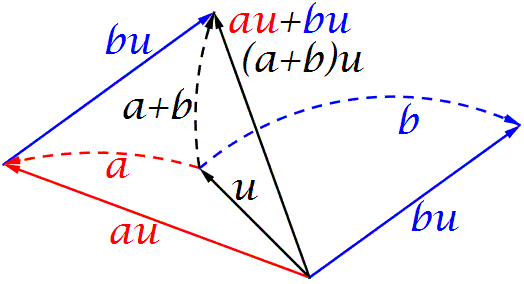
\includegraphics[width=0.5\textwidth]{imagenes/imagenes01/T01IM01.png}
		%\caption{Los dos problemas clásicos del cálculo: trazado de tangentes y áreas bajo curvas.}
	%\end{figure}
		
%varios párrafos encuadrados - explicaciones ad hoc
%\centering{
%\fbox{
%\parbox{0.95\textwidth}{
%varios
%
%$parrafos
%
%dentro
%}
%}
%}
% \justify


%\rotatebox{180}{\leftline{\textcolor{gris}{tararí}}}.


